This Chapter is using Wesson's Tokamaks as a reference. 

\section{The reaction}

The most commonly used Thermal fusion fuel is Deuterium and tritium

\begin{equation}
_{1} \mathrm{D}^{2}+_{1} \mathrm{T}^{3} \rightarrow_{2} \mathrm{He}^{4}+_0\mathrm{n}^{1}
\end{equation}

This reaction generate 17.59MeV of energy. 

%With the concentration of 1 tritium atom per $10^{17}$ water molecules, 1 deuterium atom per 3200 water molecules, 1 ton of water can generate 0.94J of energy. 

To put it into perspective, 1oz of the tritium can produce $4.4GW\cdot h$ of energy. 

\section{Power Balance}

The reaction rate can be expressed in the following way, 

\begin{equation}
\mathcal{R}=\iint \sigma\left(v^{\prime} v^{\prime} f_{1}\left(v_{1}\right) f_{2}\left(v_{2}\right) \mathrm{d}^{3} v_{1} \mathrm{d}^{3} v_{2}\right.
\end{equation}

Where $\sigma$ is the cross section and $f(v_i)$ is the distribution. For most cases, Maxwellian distribution will relatively accurately describe the distribution inside of the reactor. 

Then the reaction rate can be rewriten in the following way: 

\begin{equation}
\begin{aligned} \mathcal{R}=n_{1} n_{2} & \frac{\left(m_{1} m_{2}\right)^{3 / 2}}{(2 \pi T)^{3}} \iint \exp \left(-\frac{m_{1}+m_{2}}{2 T}\left(\mathbf{V}+\frac{1}{2} \frac{m_{1}-m_{2}}{m_{1}+m_{2}} v^{\prime}\right)\right) \\ & \times \sigma\left(v^{\prime}\right) v^{\prime} \exp \left(-\frac{\mu v^{\prime}}{2 T}\right)^{2} \mathrm{d}^{3} v^{\prime} \mathbf{d}^{3} V \end{aligned}
\end{equation}

Where $$
\mathbf{V}=\frac{v_{1}+v_{2}}{2} \quad \text { and } \quad \mu=\frac{m_{1} m_{2}}{m_{1}+m_{2}}
$$

Integrate of V, then we got, 

\begin{equation}
\mathcal{R}=\left(\frac{8}{\pi}\right)^{1 / 2} n_{1} n_{2}\left(\frac{\mu}{T}\right)^{3 / 2} \frac{1}{m_{1}^{2}} \int \sigma(\varepsilon) \varepsilon \exp \left(-\frac{\mu \varepsilon}{m_{1} T}\right) \mathrm{d} \varepsilon
\end{equation}

Where \begin{equation}
\varepsilon=\frac{1}{2} m_{1} v^{\prime 2}
\end{equation}

The thermonuclear power can be expressed in the following way:

\begin{equation}
p_{\mathrm{T}_{0}}=\frac{1}{4} n^{2}<\sigma \nu> \mathcal{E}
\end{equation}

Where $<\sigma \nu>$ is the rate of reaction. 

\subsection{Power loss}

One can determine the power loss experimentally by supply the amount of energy $P_H+P_\alpha$ such that the system has the same energy density. 

\begin{equation}
P_{\mathrm{H}}+\frac{1}{4} \overline{n^{2}\langle\sigma v)} \varepsilon_{\alpha} V=\frac{3 \overline{n T}}{\tau_{\mathrm{E}}} V
\end{equation}

Where right hand side is the power loss. 

In order to sustain the fusion, $P_H <0$ is required. Therefore, we have the criteria 

\begin{equation}
n \tau_{\mathrm{E}}>\frac{12}{\langle\sigma v\rangle} \frac{T}{\varepsilon_{\alpha}}
\end{equation}

Plugin the physical number, we have a plot as Figure \ref{fig:ignition} shown. With T=30keV, we have


\begin{figure}[h] \centering
        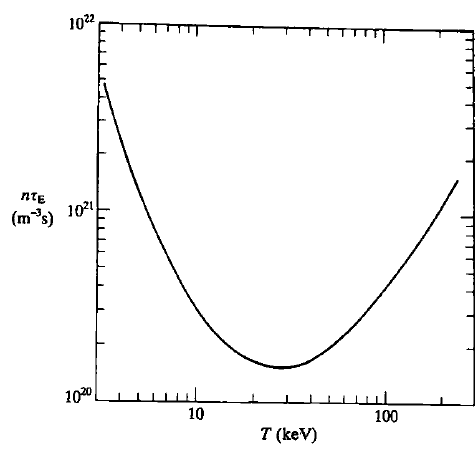
\includegraphics[width=0.4\textwidth]{Image/Ignition.png}
        \caption{$n\tau_E$ VS T}
        \label{fig:ignition}
\end{figure}

\begin{equation}
n \tau_{\mathrm{E}}>1.5 \times 10^{20} \mathrm{m}^{-3} \mathrm{s}
\end{equation}


\section{Ignition Criteria}

In order to make the reaction happen, atom has to overcome the Coulomb barrier which is just over 100keV 


\section{Confinement}

Confinement time can be expressed in the following way
\begin{equation}
    T_{confine} \propto \frac{1}{2} r^2_p
\end{equation}

Where $r_p$ is minor radius. 

\section{Heat extraction}

Impurity gives rise to radiation losses. Divertor is needed for controlled heat extraction. 

\section{Structure of Reactor}

The figure \ref{fig:reactor} shows the basic structure of tokamak reactor. 

\begin{figure}[h] \centering
        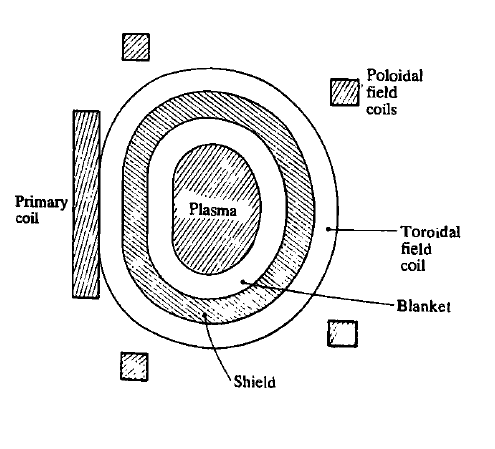
\includegraphics[width=0.4\textwidth]{Image/reactor.png}
        \caption{Structure of reactor}
        \label{fig:reactor}
\end{figure}

The blanket is used to capture neutron and convert the kinetic energy to heat in order to extract it. 